\chapter{Indledning} 
Ved ultralydsscanning af gravide er arbejdsgener hos sonograferne et kendt problem. For at udføre scanningerne holder sonograferne proben i akavede stillinger, der udsætter deres skulder, arm og håndled for store belastninger \cite{1}\cite{24}\cite{31}\cite{32}\cite{36}. Disse belastninger forøges, når et pres på mellem 3 og 11 kilo kræves for at få et klart ultralydsbillede, se Bilag 12, 28.04.2016. Disse stillinger øger risikoen for at få arbejdsskader. Grundet sonografernes belastende arbejdsstillinger er der fra Dansk Føtalmedicinsk Selskab opstillet guidelines angående det maksimale antal timer, en sonograf anbefales at foretage scanninger i løbet af en uge. Disse guidelines er på 28 timer om ugen, se Bilag 10. Dette gør, at der skal flere sonografer til for at kunne scanne det stigende antal gravide i Danmark.\cite{Foedsler}. \\
Samtidig er Danmark inde i en udvikling, der gør at antallet af overvægtige stiger \cite{Overvaegt}. Dette gør, at sonograferne skal presse med en større kraft for at få billeder af tilsvarende kvalitet frem, se Bilag 12, 28.04.2016,\cite{8}\cite{24}\cite{31}. 

Gennem en årrække er der lavet en række forskningsstudier og forsøg med robotarm til ultralydsscanning af hjertet \cite{5}. Dette er med til at underbygge, at problemstillingen er kendt, men samtidig også, at den optimale metode endnu ikke er fundet. Yderligere findes der flere forskningsstudier, der drejer sig om udviklingen af robotter til lignende opgaver \cite{5}\cite{8}\cite{18}. Dette viser, at det er et område, der investeres penge i, og hvor der er en tro på, at der er en fremtid i. 

Denne udvikling har ført til, at firmaet Robotic Ultrasound ApS er i færd med at udvikle en Ultralyds Robotarm, der formodentlig kan afhjælpe problemet. Denne robotarm styres via et joystick, således at sonograferne kan undgå at være i de akavede arbejdsstillinger, men i stedet kan styre robotten til de ønskede stillinger, se figur \ref{opstilling}.  

\begin{figure}[H]\centering
	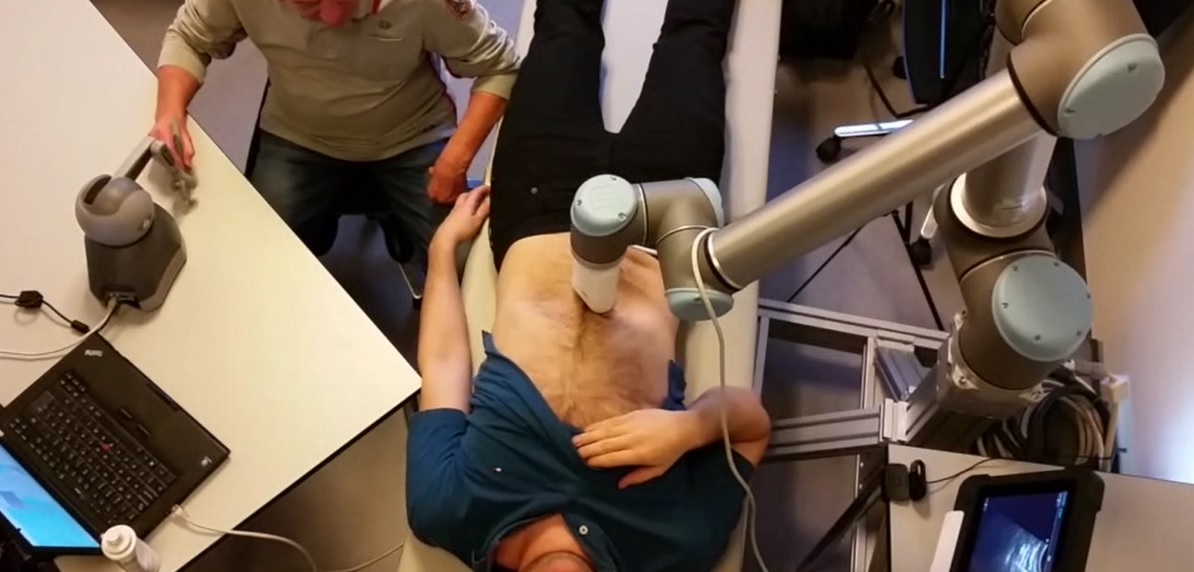
\includegraphics[width = 0.85\textwidth]{Figurer/ergonomiskLosning.jpg}
	\caption{Eksempel på opstilling af Ultralyds Robotarm. På billedet ses joystick(tv.) og robotarm(th.).  }
	\label{opstilling}
\end{figure}

%Problemstillingen i denne form er et område der ikke tidligere er afdækket. Men tidligere forskning i forhold til ultralydsscanning med robot gør at der findes tilstrækkelig videnskabelig dokumentation til at bygge mini-MTV’en op omkring. 

\section{Formål}
Formålet med denne mini-MTV er derfor at vurdere, om Ultralyds Robotarmen kan implementeres som en teknologisk aflastningsløsning for sonografer i deres arbejde med scanning af gravide. Det ønskes at klarlægge fordele og ulemper ved både de eksisterende arbejdsforhold, forholdene ved implementering af Ultralyds Robotarmen, samt hvilke forskelle robotarmen vil medføre for sonografer og gravide. \\
Dette vil blive undersøgt ved at besvare følgende opstillede MTV-spørgsmål i rapporten:
\begin{itemize}
\item Hvilke funktioner har teknologien og hvordan anvendes funktionerne?
\item Hvilke arbejdsgener oplever sonografer ved ultralydsscanning ved eksisterende procedurer og hvorledes påvirkes dette ved indførsel af teknologien?
\item Hvorledes vil afdelingernes arbejdsgange blive påvirket ved indførsel af teknologien?
\item Hvilke etiske og patientmæssige udfordringer vil der være ved at indføre teknologien?
\item Hvad vil være de økonomiske konsekvenser af at indføre teknologien i forhold til eksisterende procedurer?
\end{itemize}

Yderligere forventes det, at rapportens resultater vil blive efterspurgt forud for en beslutningstagning, når robotarmen er færdigudviklet og produceret. Dermed er formålet med mini-MTV’en også at bidrage til beslutningsgrundlaget for den enkelte sygehusafdeling, om Ultralyds Robotarmen skal implementeres, og i så fald hvilke aspekter, der skal tages højde for og medtages i en vurdering.

\section{Projektafgrænsning}
Projektet afgrænses til en vurdering af, hvorvidt det kan betale sig at gøre brug af en Ultralyds Robotarm ved scanning af gravide i forhold til det udstyr, der benyttes på afdelingerne i dag. Det primære fokus i projektet er problemstillingen om, at et stort antal sonografer oplever arbejdsgener ved scanningsarbejdet \cite{1}\cite{24}\cite{30}\cite{31}\cite{36}. \\
Rapportens fokus på sonografer er fundet ved udarbejdelse af interessentanalyse, se Bilag 14. Projekt blev afgrænset til dette fokus, da sonografer er den gruppe der foretager størstedelen af scanningerne i Danmark, hvor lægerne varetager en mindre andel af scanningerne.

Ultralyds Robotarmen åbner også for muligheden om at bruge denne som en telemedicinsk løsning, hvor selve sonografen, der foretager scanningen er placeret på et andet sygehus. Dette aspekt er fravalgt at vurdere på i denne mini-MTV. 

Opgaven er afgrænset til en 25 siders rapport, hvor det skriftlige omfang på en typisk dansk MTV ligger på over 100 sider. Dette gør, at det er en mini-MTV, der udarbejdes. I en mini-MTV vurderes problemstillingen på de fire parametre: Teknologi, Organisation, Patient og Økonomi. 

Den korte tidshorisont til udarbejdelsen af denne mini-MTV har været en afgørende faktor for, at det er valgt at begrænse projektet til at bygge på interview med to relevante danske sygehus afdelinger, samt en litteratursøgning på problemstillingen. Normalt er udarbejdelsen af en MTV en lang proces, da det kræver stort researcharbejde. Interview er afholdt med "Kvindeafdelingen, Svangre- og Ultralydsambulatorium" på Hospitalsenheden Horsens (HEH) og afdelingen "Kvindesygdomme og Fødsler" på Regionshospitalet Viborg (RMV).

\section{Projektorganisation}
Projektet er blevet udarbejdet som semesterprojekt af seks sundhedsteknologistuderende på 4. semester ved Ingeniørhøjskolen Aarhus Universitet. \\
Hovedforfattere til de enkelte kapitlerne er:
\begin{itemize}
\item Teknologi: Ditte Callesen, Ida Skovbjerg og  Mette Knudsen
\item Organisation: Anne Hoelgaard, Ida Skovbjerg og Nina Brkovic
\item Patient: Ditte Callesen, Freja Munk og Nina Brkovic
\item Økonomi: Anne Hoelgaard, Freja Munk og Mette Knudsen
\end{itemize}

\label{version_Systemark}
%\end{longtabu}